\section{Casimir forces between a conducting plate and a dielectric sphere} \label{sec:3:casimir-plate-sphere}

There does not exist a closed form expression for the Casimir energy between a dielectric sphere with radius $R$ an dielectric constant $\varepsilon_r$ in front of a conducting plate, that is applicable at all sphere-plate separations $L/R$.
In the limit of small separations, the proximity force approximation from \cref{sec:3:pfa} is valid and yields for dielectric or conducting spheres
\begin{align}\label{eq:3:casimir-sphere-plate-PFA}
  &E_\mathrm{PFA} = -\frac{\hbar c \pi^3}{720} \left(\frac{\varepsilon_r - 1}{\varepsilon_r + 1}\right)\varphi(\varepsilon_r) \frac{R}{\mathscr{L}^2} \sim \frac{1}{(L-R)^2} \quad\quad \text{for}\ L/R \approx 1 \\ \label{eq:3:casimir-sphere-plate-PFA-conducting}
  &E_\mathrm{PFA,\,cond.} = E_\mathrm{PFA}(\varepsilon_r \rightarrow \infty) = -\frac{\hbar c \pi^3}{720} \frac{R}{\mathscr{L}^2} .
\end{align}
For arbitrary separations, the Casimir energy can only be expressed as an infinite series \cite{Emig_2007,Emig_2007a} or in terms of an integral \cite{Ford_1998}
The integral form reads
\begin{multline}\label{eq:3:ford-integral}
  F = - \frac{\hbar c}{4 \pi L^4} \int_{0}^{\infty} \dd \omega \, \alpha(\omega) \left[3\sin 2 \omega L - 6L\omega \cos 2 \omega L \right. \\ 
  \left. - 6L^2\omega^2 \sin 2 \omega L + 4L^3\omega^3 \cos 2 \omega L\right].
\end{multline}
where $\alpha$ is the electric polarizability of the sphere and the integration is performed over all possible interaction frequencies $\omega$ of the electromagnetic field with the materials.

In the \emph{large-separation-limit (LSL)}, where the sphere-plate separation are much larger the the resonant wavelength of the material, the polarizability can be taken as a static constant \cite{Ford_1998,Kamp_2020}.
In this case, the integral eq. \eqref{eq:3:ford-integral} can be solved analytically by using an exponential convergence factor resulting in
\begin{equation}
  F = -\frac{6 \hbar c}{4 \pi L^5} \alpha .
\end{equation}
The polarizability of a uniform dielectric sphere with a dielectric constant $\varepsilon_r$ is calculated in \cref{apx:polarizability-sphere} and is given by
\begin{equation}\label{eq:3:polarizability-sphere}
  \alpha_\mathrm{sphere} \propto \left(\frac{\varepsilon_r - 1}{\varepsilon_r + 2}\right) R^3
\end{equation}
resulting in a Casimir energy of
\begin{align}\label{eq:3:casimir-sphere-plate-LSL}
  &E_\mathrm{LSL} = -\frac{3}{8} \frac{\hbar c}{\pi L^4} \left(\frac{\varepsilon_r - 1}{\varepsilon_r + 2}\right)R^3 \sim \frac{1}{L^4} \quad\quad\quad \text{for}\ L/R \gg 1 \\ \label{eq:3:casimir-sphere-plate-LSL-conducting}
  &E_\mathrm{LSL,\,cond.} = E_\mathrm{LSL}(\varepsilon_r \rightarrow \infty) = -\frac{3}{8} \frac{\hbar c R^3}{\pi L^4} .
\end{align}
This matches precisely the leading-order term in the series expansion from Ref. \cite{Emig_2007a} and Ref. \cite{Pirozhenko_2013}.
A comparison of the PFA and LSL approximations across all separations is shown in \cref{fig:3:casimir-behavior}, alongside numerical results from Ref \cite{Emig_2007a}.
\begin{figure}[!ht]
  \centering
  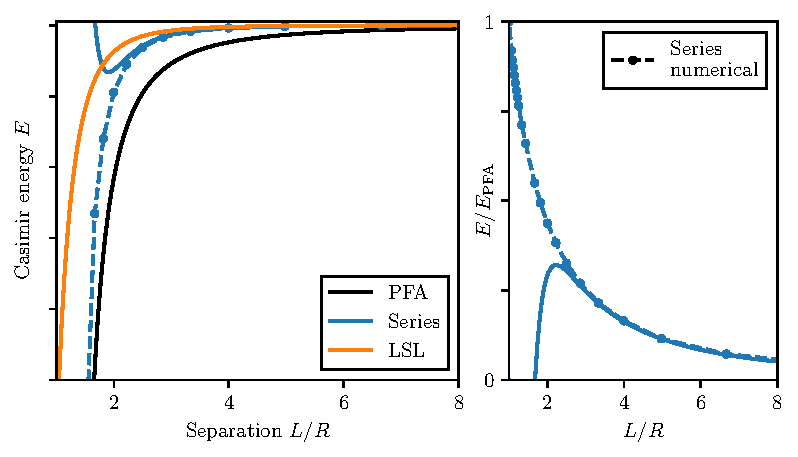
\includegraphics[width=\textwidth]{./../figures/casimir/casimir-behavior.pdf}
  \caption{Behavior of the Casimir energy for different sphere-plate separations $L/R$. For close separations ($L/R \approx 1$), the PFA eq. \eqref{eq:3:casimir-sphere-plate-PFA} is valid whereas for large separations ($L/R \gg 1$) the LSL eq. \eqref{eq:3:casimir-sphere-plate-LSL} can be used. Additionally the numeric series expansion from Ref. \cite{Emig_2007a} is shown, which converges to the PFA and LSL in each limit.}
  \label{fig:3:casimir-behavior}
\end{figure}

The scaling of $1/L^4$ for large separations can additionally be motivated empirically. Casimir and Polder calculated the potential between two atoms separated by a distance $L$ with polarizability $\alpha_i$ as \cite{Casimir_1948a} \footnote{For two macroscopic spheres, the Casimir potential looks identical to eq. \eqref{eq:3:casimir-polder-two-atoms}. The polarizability $\alpha$ is given by eq. \eqref{eq:3:polarizability-sphere}, resulting in a Casimir potential between two identical dielectric spheres in the large separation limit of $-\frac{23 \hbar c}{4\pi L^7}\left(\frac{\varepsilon_r - 1}{\varepsilon_r + 2}\right)^2R^6$ \cite{Emig_2007}.}
\begin{equation}\label{eq:3:casimir-polder-two-atoms}
  E = -\frac{23 \hbar  c \alpha_1 \alpha_2}{4 \pi L^7} .
\end{equation}
If both atoms are approximated as spheres with $\alpha \sim R^3$ and one of them is increased to the size of $R \sim L$, the total Casimir-Polder potential between them effectively scales with $\sim R^3/L^4$.
This representation corresponds to the limit $L/R \gg 1$ and aligns with the actual scaling of the macroscopic Casimir potential for large separations in eq. \eqref{eq:3:casimir-sphere-plate-LSL}.

The series expansion in \cref{fig:3:casimir-behavior} suggests, that the proximity-force-approximation is an upper bound for the actual Casimir interaction at all separations. In fact, it can be proven, that the PFA for a superconducting sphere and a plate always predicts a stronger force $\abs{\nabla E}$ than the LSL.
\begin{theorem}
  The Casimir force in the PFA-model eq. \eqref{eq:3:casimir-sphere-plate-PFA} between a superconducting sphere ($\varepsilon_r \rightarrow \infty$) and a perfectly conducting plate is an upper bound for the LSL eq. \eqref{eq:3:casimir-sphere-plate-LSL}.
\end{theorem}
\begin{proof}
  The proof is given in the following steps: \textbf{(a)} first it is shown that $\abs{\nabla E_\mathrm{PFA}} > \abs{\nabla E_\mathrm{LSL}}$ for arbitrary dielectric spheres, then it will be shown \textbf{(b)} that $\abs{\nabla E_\mathrm{PFA,\,cond.}} \geq \abs{\nabla E_\mathrm{PFA,\,diel.}}$.

  \textbf{(a)} By directly comparing the gradients of eq. \eqref{eq:3:casimir-sphere-plate-PFA} (PFA) and eq. \eqref{eq:3:casimir-sphere-plate-PFA} (LSL),  one can find
  the inequality
  \begin{align*}
    &\qquad\qquad\qquad\qquad\qquad\ \ \abs{\nabla E_\mathrm{PFA}} > \abs{\nabla E_\mathrm{LSL}} \\
    &\Longleftrightarrow \quad  \frac{2\hbar c \pi^3}{720}\left(\frac{\varepsilon_r - 1}{\varepsilon_r + 1}\right)\varphi(\varepsilon_r)\frac{R}{\mathscr{L}^3} > \frac{12 \hbar c}{8\pi L^5}\left(\frac{\varepsilon_r - 1}{\varepsilon_r + 2}\right)R^3 \\
    &\Longleftrightarrow \quad \frac{\pi^4}{540}\left(\frac{\varepsilon_r + 2}{\varepsilon_r + 1}\right)\varphi(\varepsilon_r) > \frac{(L-R)^3 R^2}{L^5} = \left(\frac{R}{L}\right)^2 - 3\left(\frac{R}{L}\right)^3 + 3\left(\frac{R}{L}\right)^4 - \left(\frac{R}{L}\right)^5
  \end{align*}
  One can easily convince oneself that the right-hand side (for $R/L \leq 1$) is upperbounded by $\approx 0.0346$ (at $R/L = 0.4$). By remembering that $(\varepsilon_r + 2)/(\varepsilon_r + 1) > 1$ and $\varphi(\varepsilon_r) \gtrsim 0.46$ one can put a lower bound on the left-hand side by $0.0830 > 0.0346$. Therefore, $\abs{\nabla E_\mathrm{PFA}} > \abs{\nabla E_\mathrm{LSL}}$.

  \textbf{(b)} By using eq. \eqref{eq:3:casimir-sphere-plate-PFA} and eq. \eqref{eq:3:casimir-sphere-plate-PFA-conducting} for the PFA of a dielectric and conducting sphere, it follows quickly that $\abs{\nabla E_\mathrm{PFA,\,cond.}} \geq \abs{\nabla E_\mathrm{PFA}(\varepsilon_r)}$, because $\varphi(\varepsilon_r)$ as well as $(\varepsilon_r - 1)/(\varepsilon_r + 1)$ are monotonically increasing with $\varepsilon_r$. 

  Combining steps \textbf{(a)} and \textbf{(b)} results in
  \begin{equation}
    \abs{\nabla E_\mathrm{PFA,\,cond.}} \geq \abs{\nabla E_\mathrm{PFA,\,diel.}} > \abs{\nabla E_\mathrm{LSL}} .
  \end{equation}
  Thus, the PFA provides an upper bound for the Casimir force at all separations.
  Considering the numerical series expansion, it appears as if the argument applies at all separations $L/R$ - although this is not mathematically proven here.
\end{proof}
\begin{remark}
  For later calculations, only the difference in the Casimir energy for slightly different separations $L$ and thus effectively the gradient $\nabla E = \dd E / \dd L$ is required. Thus, the proof was given in terms of the Casimir force $F= -\nabla E$.
\end{remark}

For subsequent calculations, the PFA is therefore used as a worst-case approximation of the Casimir energy. Whenever possible, results are cross-verified anc compared with the LSL model.